

\SaveVerb{py_full}|x.merge(y, how='outer')|
\SaveVerb{py_inner}|x.merge(y, how='inner')|
\SaveVerb{py_left}|x.merge(y, how='left')|
\SaveVerb{py_right}|x.merge(y, how='right')|
\SaveVerb{r_full}|full_join(x,y)|
\SaveVerb{r_inner}|inner_join(x,y)|
\SaveVerb{r_left}|left_join(x,y)|
\SaveVerb{r_right}|right_join(x,y)|


\begin{table}
  \begin{tabularx}{\linewidth}{llXll}
    \toprule
    Type & Result & Description  & R & Python \\
    \midrule

    Outer & 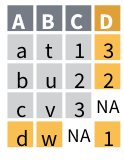
\includegraphics[height=5em,valign=t]{figures/wrangling_full} & All units from both sets &
    \UseVerb{r_full} & \UseVerb{py_full} \\

    Inner & 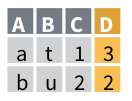
\includegraphics[height=3em,valign=t]{figures/wrangling_inner} & Only units that are in both sets &
    \UseVerb{r_inner} & \UseVerb{py_inner} \\

    Left & 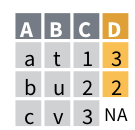
\includegraphics[height=4em,valign=t]{figures/wrangling_left} & All units from left-hand set &
    \UseVerb{r_left} & \UseVerb{py_left} \\

    Right & 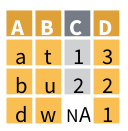
\includegraphics[height=4em,valign=t]{figures/wrangling_right} & All units from right-hand set &
    \UseVerb{r_right} & \UseVerb{py_right} \\
    
    \bottomrule

  \end{tabularx}
  \raggedright Joining data sets |x| and |y| on shared key columns |A| and |B|: 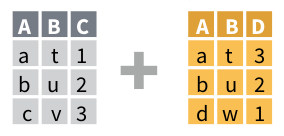
\includegraphics[height=4em]{figures/wrangling_joins} \\ Images CC-BY-SA RStudio (TODO:recreate images to avoid problems due to SA)
  \caption{Different join types}
  \end{table}
